\chapter{Childline}
\ifpdf
    \graphicspath{{Chapter2/Chapter2Figs/PNG/}{Chapter2/Chapter2Figs/PDF/}{Chapter2/Chapter2Figs/}}
\else
    \graphicspath{{Chapter2/Chapter2Figs/EPS/}{Chapter2/Chapter2Figs/}}
\fi

\section{About Childline}
% \markboth{\MakeUppercase{\thechapter. My Second Chapter }}
In 1996, CHILDLINE India Foundation (CIF) launched CHILDLINE, the country's first toll-free tele-helpline for street children in distress. As of March 2014, total of 31 Million calls since inception have been serviced by CHILDLINE service and operates in 291 cities/districts in 31 States and UTs through its network of over 540 partner organizations across India.

\begin{figure}[ht!]
  \begin{center}
    \leavevmode
    \ifpdf
      
\includegraphics[height=1in]{1098}
    \else
      
\includegraphics[bb = 92 86 545 742, height=6in]{1098}
    \fi
    \caption{1098: Childline}
    \label{FigAir}
  \end{center}
\end{figure}



\begin{figure}
  \begin{center}
    \leavevmode
    \ifpdf
      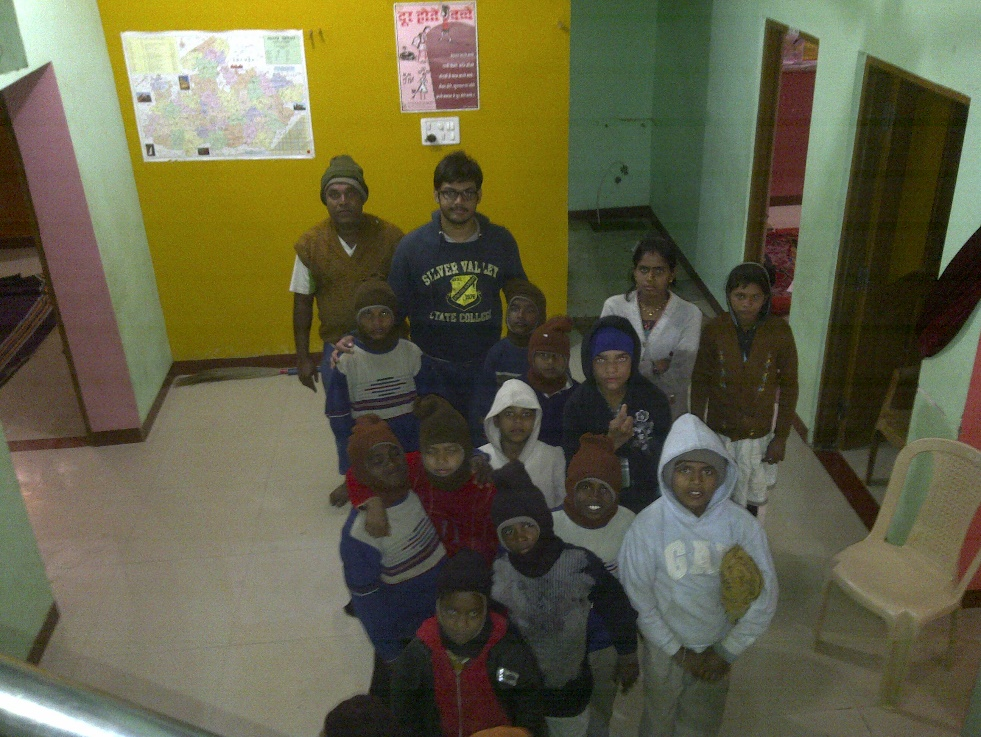
\includegraphics[height=3.5in]{childlinekids}
    \else
      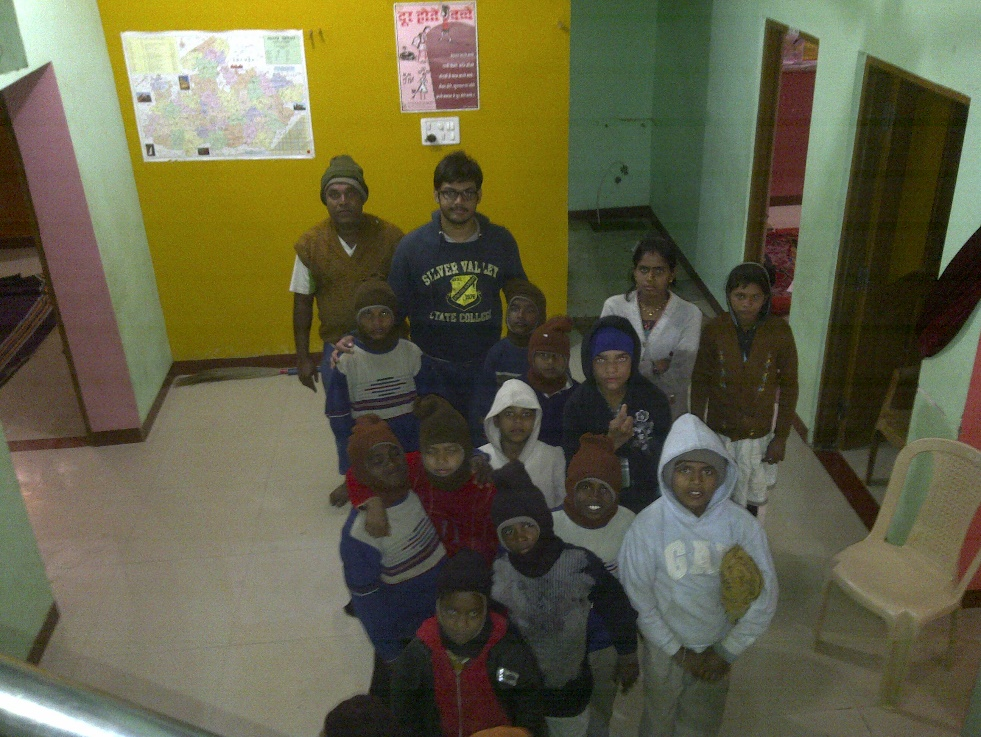
\includegraphics[bb = 92 86 545 742, height=6in]{childlinekids}
    \fi
    \caption{Open Shelter Kids}
    \label{FigAir}
  \end{center}
\end{figure}

\section{Involvement of Synergy Sansthan}
% \markboth{\MakeUppercase{\thechapter. My Second Chapter }}
Synergy Sansthan is a partner organization of Childline. When a person reports a case on 1098 in the Hard district or neighboring areas, the information is forwarded to it. Then the on duty official from Synergy Sansthan has to go and rescue the child in 6 hours. The child would then be living in the open shelter till legal action is taken. The magistrate decides the fate of the child if he or she is to be sent to a guardian, continue living in the open shelter or sent to an orphanage. Synergy Sansthan does proper counseling of the children so that they can get accustomed easily. Most of the children there come from very harsh and difficult backgrounds which can only be dealt with properly by professionals.



\section{Some case studies}
\subsection{Jalim Singh}
Jalim lived with his grandmother and worked at a hotel, his grandmother had no source of income other than her pension. His father was in prison and his mother had expired. Hence the financial status of the family was very poor. He had many vices like consuming tobacco, drinking, taking narcotics etc. He was also disrespectful to elders, used abusive language and picked up fights. His grandmother wanted him to study and enroll him in a school but was unable to do so. When we informed her about the open shelter and that the children were given a good place to stay, given proper food and exercise she agreed readily.
% \vspace{1cm}

\begin{figure}
  % \begin{flushleft}
  %   \leavevmode
  %   \ifpdf
  %     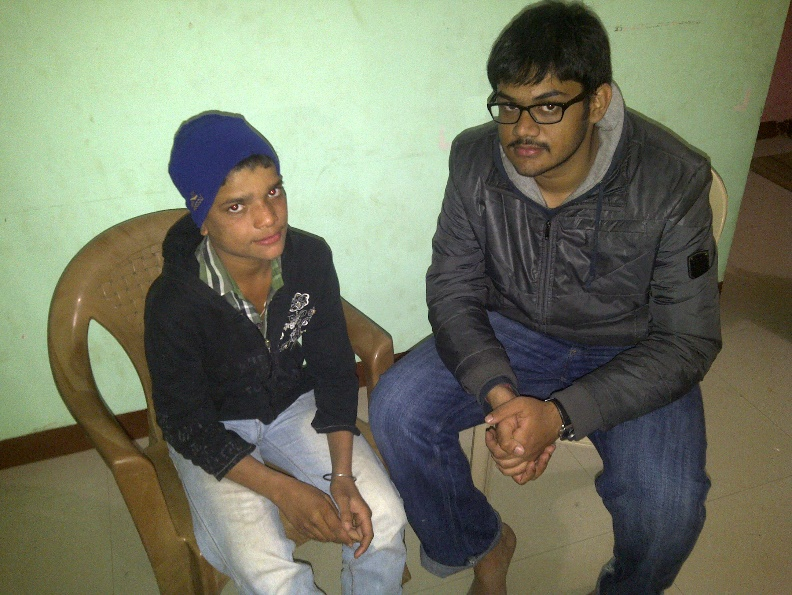
\includegraphics[height=2in]{jalimsingh}
  %   \else
  %     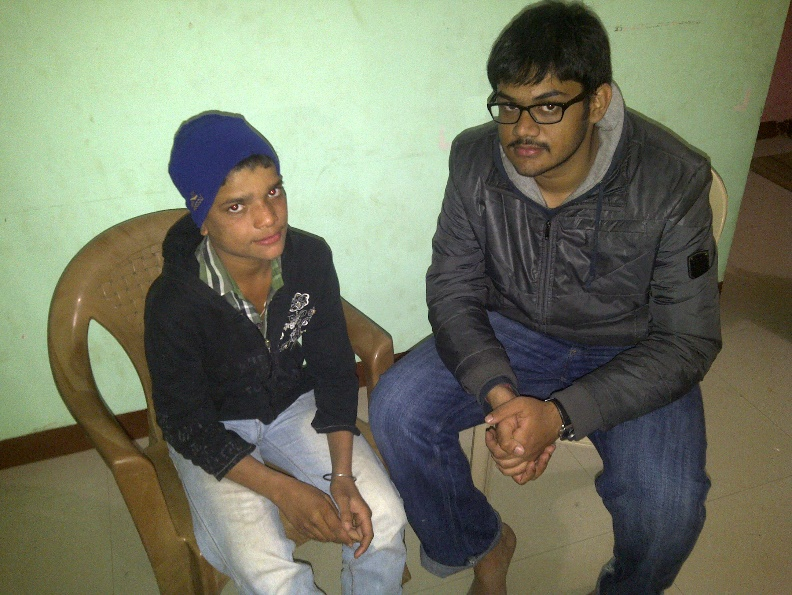
\includegraphics[bb = 92 86 545 742, height=6in]{jalimsingh}
  %   \fi
  %   \caption{Talking to Jalim Singh}
  %   \label{FigAir}
  % \end{flushleft}
  % \begin{flushright}
  %   \leavevmode
  %   \ifpdf
  %     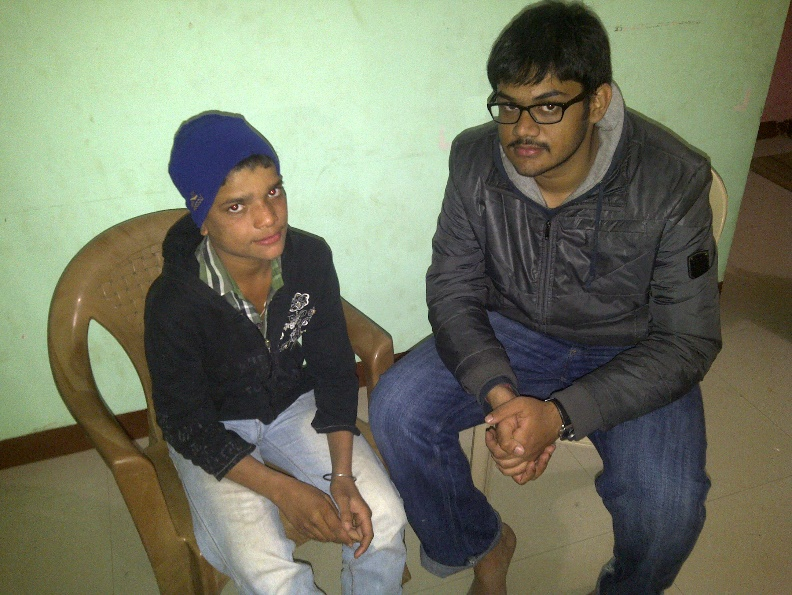
\includegraphics[height=2in]{jalimsingh}
  %   \else
  %     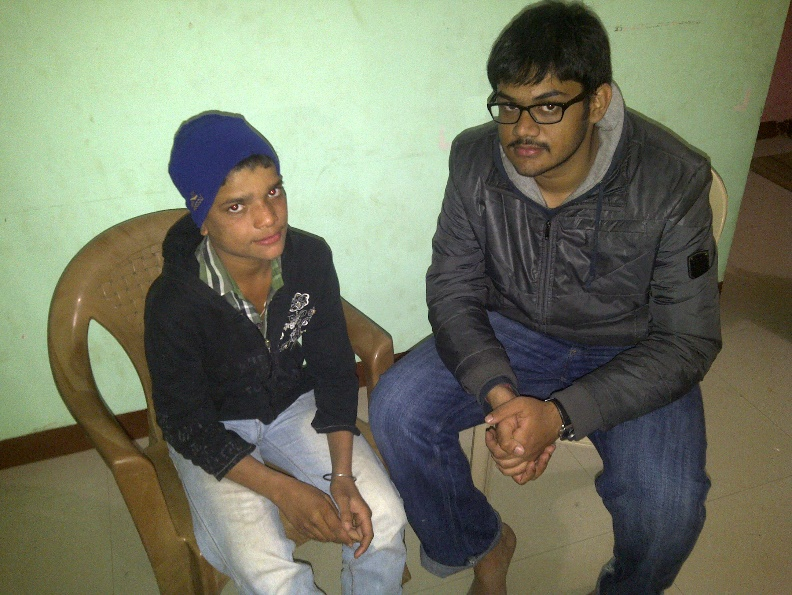
\includegraphics[bb = 92 86 545 742, height=6in]{jalimsingh}
  %   \fi
  %   \caption{Talking to Jalim Singh}
  %   \label{FigAir}
  % \end{flushright}


	\centering
	\begin{subfigure}{.5\textwidth}
	  	\centering
	  	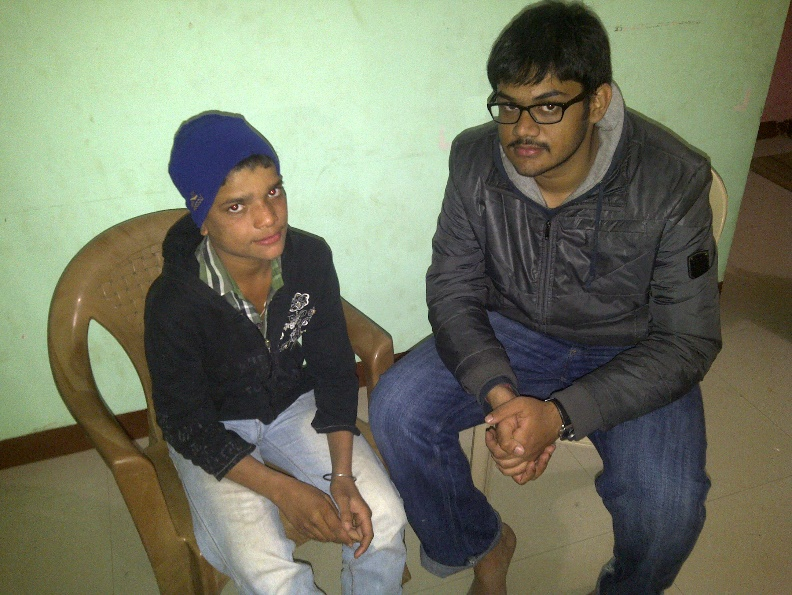
\includegraphics[width=2.5in]{jalimsingh}
	  	\caption{Jalim Singh}
	  	\label{fig:sub1}
	\end{subfigure}%
	\begin{subfigure}{.5\textwidth}
	  	\centering
	  	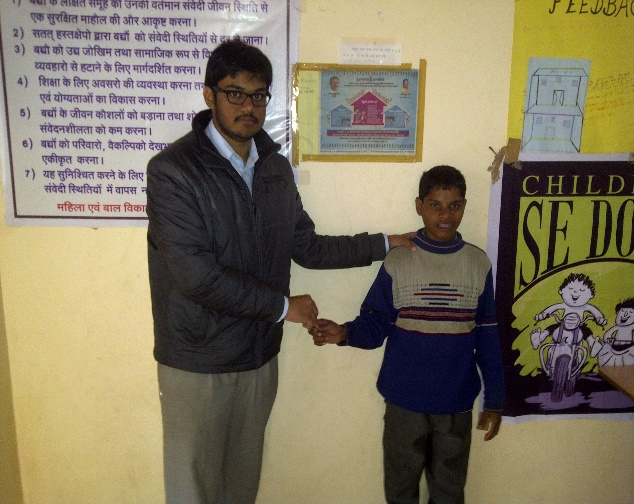
\includegraphics[width=2.5in]{othekid}
	  	\caption{Lokesh}
	  	\label{fig:sub2}
	\end{subfigure}
	\caption{Jalim and Lokesh - Case Studies}
	\label{figstart}


\end{figure}

After staying at Synergy Sansthan, he developed a lot of positive changes. As he was the eldest among all kids, he developed leadership skills. He has left all drugs and forms of intoxication. He was given proper counseling so that he could mend his ways properly. He goes to school regularly and is enjoying his life now.
\subsection{Lokesh}
Lokesh was a resident of Beragarh. The status of the family was pitiable, his parents had been murdered and his grandfather took care of him, his uncle and aunt stayed somewhere else, the grandfather was blind and to support the household Lokesh had to become a rag picker instead of going to school. If the income was very low his grandfather commanded him to steal. One day he was caught stealing and the shopkeeper took him to the police station. The police then informed the Child-line team about Lokesh and they took him to the ``open shelter''. During counseling the Child-line team got to know that Lokesh had many bad habits like abusing, fighting, shouting and disobeying elders.

% \begin{figure}
%   \begin{flushleft}
%     \leavevmode
%     \ifpdf
%       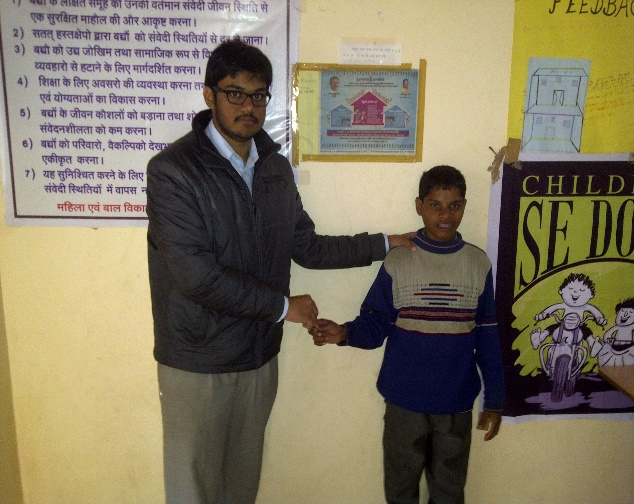
\includegraphics[height=2in]{othekid}
%     \else
%       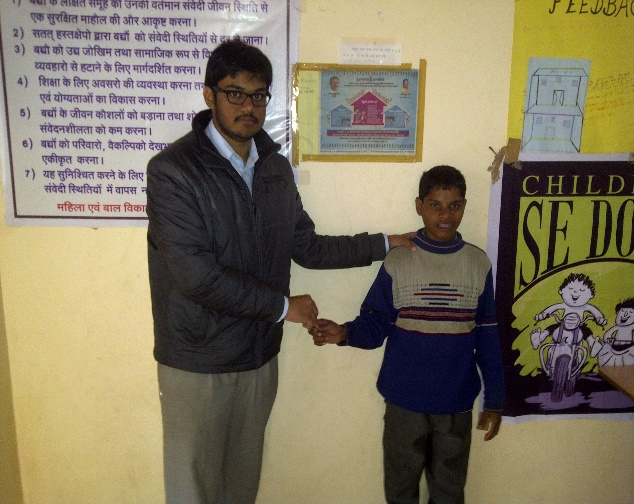
\includegraphics[bb = 92 86 545 742, height=6in]{othekid}
%     \fi
%     \caption{Talking to Lokesh}
%     \label{FigAir}
%   \end{flushleft}
% \end{figure}


After staying at Synergy Sansthan lots of positive changes happened with him. He has started going to school regularly and is enjoying it. He likes to play football most amongst all sports. 
% \subsection{first subsection in the Second Section}
% ... and some more ...

% \subsection{second subsection in the Second Section}
% ... and some more ...

% \subsection{third subsection in the Second Section}
% ... and some more ...


% ------------------------------------------------------------------------

%%% Local Variables: 
%%% mode: latex
%%% TeX-master: "../thesis"
%%% End: 
